%  !TeX  root  =  user_guide.tex

\chapter{Working with Raster Data}\label{label_raster}
\index{raster layers|(}

% when the revision of a section has been finalized, 
% comment out the following line:
%\updatedisclaimer

This Section describes how to visualize and set raster layer properties.
QGIS supports a number of different raster formats. Currently tested formats
include:\index{raster layers!data formats}

\begin{itemize}[label=--]
\item Arc/Info Binary Grid
\item Arc/Info ASCII Grid
\item GRASS Raster
\item GeoTIFF
\item JPEG
\item Spatial Data Transfer Standard Grids (with some limitations)
\item USGS ASCII DEM
\item Erdas Imagine
\end{itemize}

Because the raster implementation in QGIS is based on the GDAL library, other
raster formats implemented in GDAL are also likely to work - if in doubt try 
to open a sample and see if it is supported. You find more details about GDAL 
supported formats in Appendix \ref{appdx_gdal}
\index{raster layers!GDAL implementation} or at 
\url{http://www.gdal.org/formats_list.html}. If you want to load GRASS raster 
data, please refer to Section~\ref{sec:load_grassdata}.

\section{What is raster data?}\label{label_whatsraster}
\index{raster layers!definition}

Raster data in GIS are matrices of discrete cells that represent features on,
above or below the earth's surface. Each cell in the raster grid is the same
size, and cells are usually rectangular (in QGIS they will always be
rectangular). Typical raster datasets include remote sensing data such as
aerial photography or satellite imagery and modelled data such as an elevation
matrix.

Unlike vector data, raster data typically do not have an associated database
record for each cell. They are geocoded by its pixel resolution and the x/y 
coordinate of a corner pixel of the raster layer. This allows QGIS to position 
the data correctly in the map canvas. 

QGIS makes use of georeference information inside the raster layer (e.g. GeoTiff) 
or in an appropriate world file to properly display the data.\index{raster layers!georeferenced}
	
\section{Loading raster data in QGIS}\label{label_loadraster}

Raster layers are loaded either by clicking on the 
\toolbtntwo{mActionAddRasterLayer}{Load Raster} icon or by
selecting the \mainmenuopt{View} > \dropmenuopttwo{mActionAddRasterLayer}{Add Raster Layer} 
menu option. More than one layer can be loaded at the same time by holding down the
\keystroke{Control} or \keystroke{Shift} key and clicking on multiple items 
in the dialog \dialog{Open a GDAL Supported Raster Data Source}.\index{raster layers!loading}

Once a raster layer is loaded in the map legend you can click on the layer name with the 
right mouse button to select and activate layer specific features or to open 
a dialog to set raster properties for the layer.

\minisec{Right mouse button menu for raster layers}

\begin{itemize}[label=--]
\item \dropmenuopt{Zoom to layer extent}
\item \dropmenuopt{Zoom to best scale (100\%)}
\item \dropmenuopt{Show in overview}
\item \dropmenuopt{Remove}
\item \dropmenuopt{Properties}
\item \dropmenuopt{Rename}
\item \dropmenuopt{Add Group}
\item \dropmenuopt{Expand all}
\item \dropmenuopt{Collapse all}
\item \dropmenuopt{Show file groups}
\end{itemize}
	
\section{Raster Properties Dialog}\label{label_rasterprop}

To view and set the properties for a raster layer, double click 
on the layer name in the map legend or right click on the layer name and choose 
\dropmenuopt{Properties} from the context menu:\index{raster layers!context menu}
Figure \ref{fig:raster_properties} shows the \dialog{Raster Layer Properties} dialog. 
There are several tabs on the dialog: 

\begin{itemize}[label=--]
 \item \tab{Symbology}
 \item \tab{Transparency}
 \item \tab{Colormap}
 \item \tab{General}
 \item \tab{Metadata}
 \item \tab{Pyramids}
 \item \tab{Histogram}
\end{itemize}

\begin{figure}[h]
  \centering
   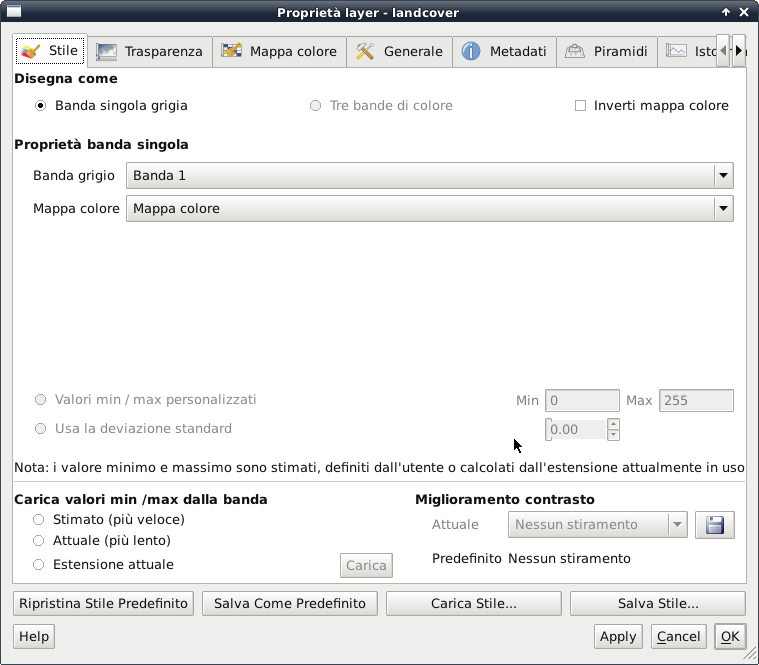
\includegraphics[clip=true, width=14cm]{rasterPropertiesDialog}
   \caption{Raster Layers Properties Dialog \nixcaption}\label{fig:raster_properties}
\end{figure}

\subsection{Symbology Tab}\label{label_sombology}

QGIS can render raster layers in two different ways :\index{raster layers!supported channels}

\begin{itemize}[label=--]
\item Single band - one band of the image will be rendered as gray or in 
pseudocolors.
\item Three band color - three bands from the image will be rendered, each 
band representing the red, green or blue component that will be used to create 
a color image.
\end{itemize}

Within both render types you can invert the color output using the 
\checkbox{Invert color map} checkbox.

\minisec{Single Band Rendering}

This selection offers you two possibilites to choose. At first you can
select which band you like to use for rendering (if the dataset has more than 
one band). 

The second option offers a selection of available colortables for rendering.

The following settings are available through the dropdownbox
\selectstring{color map}{Grayscale}, where grayscale is the default
setting.
Also available are
\begin{itemize}[label=--]
\item Pseudocolor
\item Freak Out
\item Colormap
\end{itemize}

When selecting the entry \selectstring{color map}{Colormap}, the tab
\tab{Colormap} becomes available. See more on that at chapter
\ref{label_colormaptab}.

QGIS can restrict the data displayed to only show cells whose values are
within a given number of standard deviations of the mean for the
layer.\index{raster layers!standard deviation} This is useful when you have one or
two cells with abnormally high values in a raster grid that are having a
negative impact on the rendering of the raster. This option is only available
for pseudocolor images.

\minisec{Three band color}

This selection offers you a wide range of options to modify the appereance
of your rasterlayer. For example you could switch color-bands from the
standard RGB-order to something else.

Also scaling of colors are available.


\begin{Tip}\caption{\textsc{Viewing a Single Band of a Multiband Raster}}
If you want to view a single band (for example Red) of a multiband
image, you might think you would set the Green and Blue bands to ``Not
Set''. But this is not the correct way. To display the Red band, 
set the image type to grayscale, then select Red as the band to use for Gray.
\end{Tip} 

\subsection{Transparency Tab} \label{rastertab:transparency}

QGIS has the ability to display each raster layer at varying transparency
levels.\index{raster layers!transparency} Use the transparency slider to indicate to
what extent the underlying layers (if any) should be visible though the
current raster layer. 
This is very useful, if
you like to overlay more than one rasterlayer, e.g. a shaded relief-map
overlayed by a classified rastermap. This will make the look of the map
more three dimensional.

Additionally you can enter a rastervalue, which should be treated as
{\em NODATA}.

An even more flexible way to customize the transparency can be done in the
\guiheading{Custom transparency options} section.
The transparency of every pixel can be set in this tab.

As an example we want to set the water of our example rasterfile
\filename{landcover.tif} to a transparency of 20\%. The following steps
are neccessary:
\begin{enumerate}
 \item  Load the rasterfile \filename{landcover}
 \item Open the \dialog{properties} dialog by double-clicking on the
 rasterfile-name in the legend or by right-clicking and choosing
 \dropmenuopt{Properties} from the popup meun.
 \item select the \tab{Transparency} tab
 \item \label{enum:add} Click the \toolbtntwo{mActionNewAttribute}{Add values manually}
 button. A new row will appear in the pixel-list.
 \item \label{enum:transp} enter the raster-value (we use 0 here) and adjust the
 transparency to 20\%
 \item press the \button{Apply} button and have a look at the map
\end{enumerate}

You can repeat the steps \ref{enum:add} and \ref{enum:transp} to adjust
more values with custom transparency.

As you can see this is quite easy to set custom transparency, but it can be
quite a lot of work. Therefore you can use the button
\toolbtntwo{mActionFileSave}{Export to file} to save your
transparency-list to a file. The button
\toolbtntwo{mActionAddRasterLayer}{Import from file} loads your
transparency-settings and applies them to the current rasterlayer.

\subsection{Colormap} \label{label_colormaptab}
% FIXME: Write me

The \tab{Colormap} tab is only available, when you have selected a
single-band-rendering within the tab \tab{Symbology} (see chapt. \ref{label_sombology}).

Three ways of color interpolation are available:
\begin{itemize}[label=--]
\item Discrete
\item Linear 
\item Exact
\end{itemize}

The button \button{Add Entry} adds a color to the individual color-table.
Double-Clicking on the value-column lets you inserting a specific value.
Double clicking on the color-column opens the dialog \dialog{Select
color} where you can select a color to apply on that value.

Alternatively you can click on the button
\toolbtntwo{mActionNewAttribute}{Load colormap from Band}
, which tries to
load the table from the band (if it has any).

The block \guiheading{Generate new color map} allows you to create newly
categorized colormaps. You only need to select the \selectnumber{number of
classes}{15} you need and press the button \button{Classify}. Currently
only one \selectstring{Classification mode}{Equal Interval} is
supported\index{raster layer!classify}.

\subsection{General Tab}\label{label_generaltab}

The \tab{General} tab displays basic information about the selected raster,
including the layer source and  display name in the legend (which can be
modified). This tab also shows a thumbnail of the layer, its legend symbol,
and the palette.\index{raster layers!properties}

Additionally scale-dependent visability can be set in this tab. You need to
check the checkbox and set an appropriate scale where your data will be
displayed in the map canvas.

Also the spatial reference system is printed here as a PROJ.4-string. 
This can be modified by hitting the \button{Change} button.

\subsection{Metadata Tab}\label{label_metatab}

The \tab{Metadata} tab displays a wealth of information about the raster layer,
including statistics about each band in the current raster layer. Statistics
are gathered on a 'need to know' basis, so it may well be that a given layers
statistics have not yet been collected.\index{raster layers!metadata}

This tab is mainly for information. You cannot change any values printed
inside this tab. To update the statistics you need to change to tab
\tab{Histogram} and press the button \button{Refresh} on the bottom right,
see ch. \ref{label_histogram}.

\subsection{Pyramids Tab}\label{raster_pyramids}

Large resolution raster layers can slow navigation in QGIS. By creating lower
resolution copies of the data (pyramids), performance can be considerably
improved as QGIS selects the most suitable resolution to use depending on the
level of zoom.
\index{raster layers!pyramids}
\index{raster layers!resolution pyramids}

You must have write access in the directory where the original data is stored
to build pyramids. \\
Several resampling methods can be used to calculate the pyramides:
\begin{itemize}[label=--]
\item Average
\item Nearest Neighbour
\end{itemize}

When checking the checkbox \checkbox{Build pyramids internally if
possible} QGIS tries to build pyramids internally.

Please note that building pyramids may alter the original data file and once
created they cannot be removed. If you wish to preserve a 'non-pyramided'
version of your raster, make a backup copy prior to building pyramids.

\subsection{Histogram Tab}\label{label_histogram}

The \tab{Histogram} tab allows you to view the distribution\index{raster layers!histogram} 
of the bands or colors in your raster. You must first generate the raster statistics 
by clicking the \button{Refresh} button. You can choose which bands to display by 
selecting them in the list box at the bottom left of the tab. Two different
chart types are allowed: 

\begin{itemize}[label=--]
\item Bar chart
\item Line graph
\end{itemize}

You can define the number of chart columns to use and decide whether you want 
to \checkbox{Allow approximation} or display \checkbox{out of range} values 
Once you view the histogram, you'll notice that the band statistics have been
populated on the \tab{metadata} tab.\index{raster layers!metadata)}

\begin{Tip}\caption{\textsc{Gathering Raster Statistics}}
To gather statistics for a layer, select pseudocolor rendering and
click the \button{Apply} button. Gathering statistics for a layer can be time
consuming. Please be patient while QGIS examines your
data!\index{raster layers!statistics}
\end{Tip}

\FloatBarrier
